\chapter{Proposed method}\label{ch:proposed_method}
As we pointed out in the previous chapter, human pose estimation is a problem that can be approached from a multitude of different perspectives. After extensively reviewing previous work in the field, and taking into account the particular requirements of robotics applications, we propose a very lightweight solution for 3D estimation from RGBD data that builds upon some of the methods presented in Section~\ref{subsec:dl_2d_estimation}. In this chapter, we present an overview of our system and its components. We have split our process into two major blocks: 2D and 3D estimation. For the former, three 2D human pose estimators have been tested. First, their architectures and training strategies are described and their pros and cons are discussed. Then, our method for getting 3D estimations from 2D coordinates is presented with greater detail, showing how each individual step works and how they contribute to the overall system performance. 

\section{System design}
As previously stated in Section~\ref{sec:goals}, our main objective is to build a system for 3D human pose estimation that is lightweight enough to be embedded in a robot and that can operate independently of the point of view, while perceiving in real-time the poses of the humans around. Keeping these requirements in mind, we have decided to design a hybrid system that relies on \gls{sota} \gls{dl}-based solutions for 2D human pose estimation and a very straight-forward method for augmenting the estimated 2D keypoints to 3D, leveraging the depth information provided by an RGBD sensor. An overview of this system is shown in Figure~\ref{fig:system_design}.

\begin{figure}[h]
    \centering
    \includesvg[width=\textwidth]{figures/system_design_v02.svg}
    \caption{Overview of the pipeline proposed for 3D human pose estimation.}
    \label{fig:system_design}
\end{figure}

Our method does not make any assumption on the kind of algorithm used for estimating the 2D coordinates, and so one can choose the 2D human pose estimator that better fits the particular application being developed. This flexibility allows the user to prioritize accuracy over computational cost or vice versa. It also ensures that our pipeline can be updated with novel solutions for 2D pose estimation that might be proposed in the years to come. It is important to mention that human detection is a required step before most of the available 2D pose estimators in the literature, but this step is out of the scope of this work, as there are some methods that might perform human and pose detection jointly~\cite{cao2018openpose}. For completeness, we will present a briefly description of how we achieve human detection in the next section, without going into great detail.

Regarding the 2D to 3D estimation step, we will assume that a commercial RGBD sensor is available. This is a reasonable assumption taking into account how widespread and affordable some of these sensors have become in the last years. Such is the case of the \emph{Asus Xtion} sensor~\cite{xtion}, which we will use to experimentally validate our system in Section~\ref{sec:demo}. Our proposed method for estimating the 3D coordinates from the detected 2D keypoints relies on classic computer vision techniques that are well established and that fulfill our requirements in terms of computational costs. Furthermore, the only specific step for human pose estimation in this method is the outlier rejection, and so it can be easily adapted for any kind of 3D estimation given its 2D counterparts.

\section{2D Estimation}\label{sec:2d_estimation}
In order to estimate the initial 2D locations of the human joints considered, we have evaluated the usage of three different \gls{dl}-based solutions, which have provided good results in the literature. None of them make use of explicit graphical models. The tested methods have been chosen both for their performance, in terms of the leap forward they represented for the human pose estimation field, and their intuitiveness, which will be useful to ensure a clear analysis of the results obtained. Before presenting these methods, we will start by addressing how human detection can be performed for further improving the pose estimation results.

\subsubsection{Human detection}\label{subsubsec:human_detection}
Human detection is a well studied area of computer vision, which can be considered a subfield of the more generic object detection problem. Detecting humans in 2D images is specially challenging due to the variable appearance a human body can take when projected in a 2D surface, which is highly dependent on properties like pose and clothing. We are not going to dive deep into human detection literature, but it is worth mentioning the classic approach proposed by Dalal and Triggs~\cite{dalal2005histograms}, as it is probably one of the most relevant works in the field. In their work, they build a grid of \emph{Histograms of Oriented Gradients} and classify the resulting patches using \emph{Support Vector Machines}. This is a very efficient method and, for years, it has been established as the go-to solution for human detection.

However, as it has happened for most of the classic problems in computer vision, \gls{dl} solutions have demonstrated to be far more accurate. This is specially true in the case of human detection, as there is huge availability of potential training data. Taking that into account, we have used an \emph{SSDLite MobileNetV2} model as our baseline human detector~\cite{sandler2018mobilenetv2}. It is not only precise enough for our application, but it also has been specifically built to be as lightweight as possible to ensure it is suitable for being embedded in systems with scarce resources, hence the \emph{mobile} prefix in its name. This model is based on the successful \emph{Single Shot Multibox Detector}, initially introduced by Liu \etal\cite{liu2016ssd} (see Figure~\ref{fig:ssd}), but tweaked with a novel layer that uses depth-wise separable convolutions to improve the efficiency of the model by reducing the number of parameters and operations needed during inference. The trained model is publicly available as part of the \emph{TesorFlow Model Garden}~\footnote{\url{https://github.com/tensorflow/models/tree/master/research/slim/nets/mobilenet}}.

\begin{figure}[h]
    \centering
    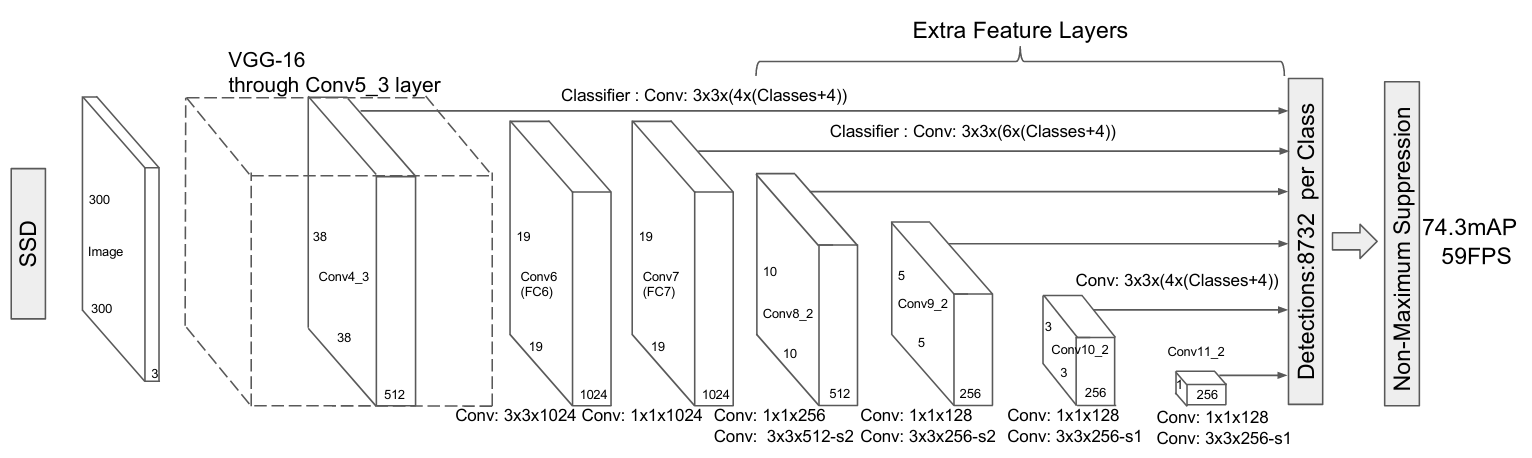
\includegraphics[width=\textwidth]{figures/ssd.png}
    \caption{\emph{Single Shot Multibox Detector} architecture as presented by Liu \etal\cite{liu2016ssd}. In the \emph{SSDLite MobileNetV2} adaptation, the convolutional layers are replaced by the depth-wise separable convolutions proposed in ~\cite{sandler2018mobilenetv2}.}
    \label{fig:ssd}
\end{figure}

\subsection{Convolutional Pose Machines}\label{subsec:cmps}
\glspl{cpm}, introduced by Wei \etal in~\cite{Wei2016-rb}, is one of the most prominent works in the 2D human pose estimation field, as it laid the foundation for the \emph{OpenPose} suite (see Section~\ref{subsec:dl_2d_estimation}). Broadly speaking, the architecture proposed by Wei \etal is a combination of multi-class predictors organized into several stages. Each of these multi-class predictors is built as a \gls{cnn} estimating the location of a single human joint. The image features and belief maps produced by each of these predictors in one stage are used as input for the next one. With each subsequent stage, the receptive field over the input image increases, implicitly encoding contextual information and allowing the network to learn correlations between parts. This effect is well exemplified in Figure~\ref{fig:cpms}, which summarizes the \glspl{cpm} architecture and shows the receptive field at different stages for an example image. In the original article, results are reported for a \gls{cpm} composed of 6 stages.

\begin{figure}[h]
    \centering
    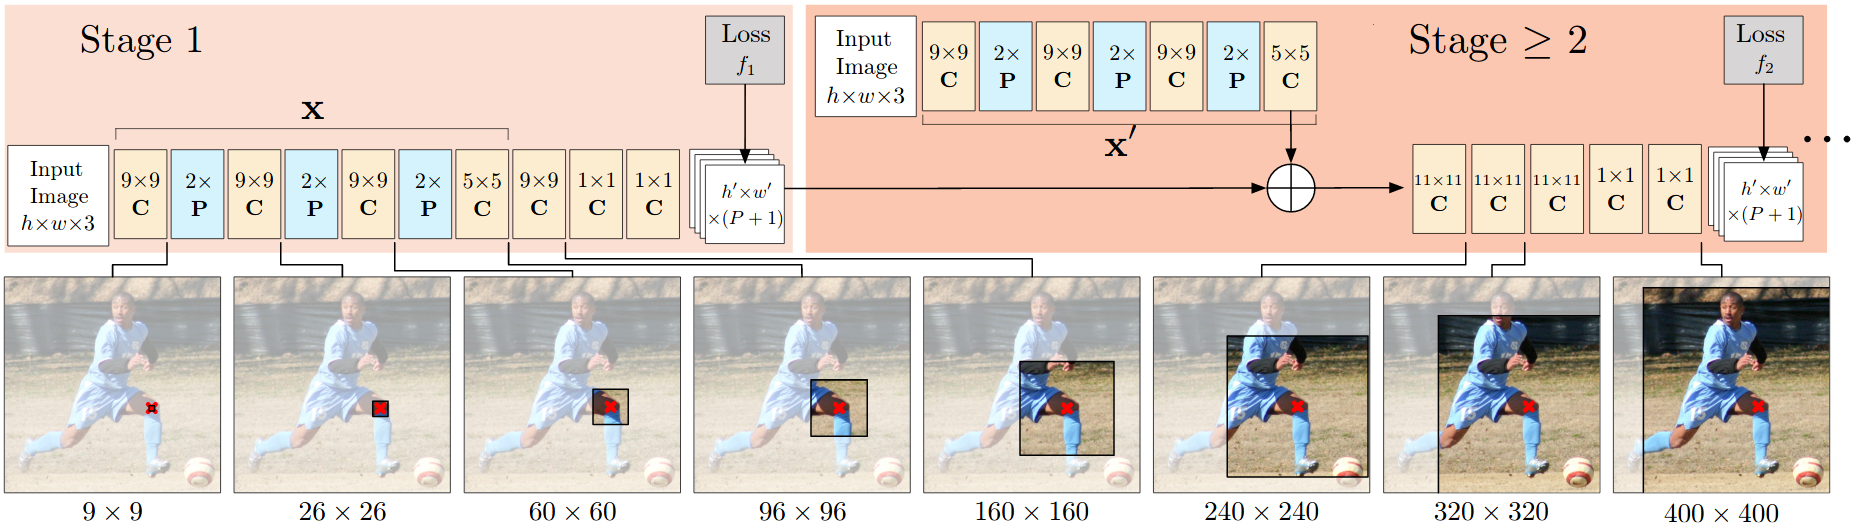
\includegraphics[width=\textwidth]{figures/cpms.png}
    \caption{Overview of the CPMs model proposed by Wei \etal\cite{Wei2016-rb}. The top of the diagram shows the architecture of the first stage and the subsequent ones. In the bottom, the increment in the receptive field across each new stage is shown.}
    \label{fig:cpms}
\end{figure}

Regarding the model training, each stage and body part has its own specific loss function, computed as the squared error between the predicted and the target belief maps. It is worth clarifying that the target belief map of each body part is created by locating a \emph{Gaussian} function at the ground-truth location. The individual losses that we have just described are then aggregated to provide the overall loss of the \gls{cpm} being trained. In that way, all the weights involved in each of the stages and predictors can be jointly trained with intermediate supervision. During evaluation, input images are cropped in a square around the subject of interest and normalized to a size of 368x368 pixels.

\subsection{Stacked Hourglass}\label{subsec:sh}
Newell \etal\cite{Newell2016-cy} propose a novel \gls{cnn} architecture, which leverage features in the image at different scales by repeated \emph{bottom-up} and \emph{top-down} processing steps, \ie from high to low resolution and vice versa, respectively. Each of these \emph{bottom-up} and \emph{top-down} blocks are given the name of \emph{Hourglass Modules}. For the \emph{bottom-up} stage, the images are downsampled by stacking several convolutional and \emph{Max Pooling} layers. For the \emph{top-down} stage, the lowest resolution image passes through several \emph{Nearest Neighbors} upsampling layers until the original resolution is reached. Each \emph{Hourglass Module} is symmetrical and the combination of features at different scales is enforced by elementwise additions between maps of equal resolution from the \emph{top-down} and \emph{bottom-up} halfs of the module. In Figure~\ref{fig:sh}, the architecture of a single \emph{Hourglass Module} is shown in a very intuitive way. In order to further consolidate the multi-scale features extracted by the \gls{cnn} and refine the estimated locations for each joint, several of these modules are stacked together. Newell \etal report their final results for a \gls{sh} model composed of 8 \emph{Hourglass Modules}.

\begin{figure}[h]
    \centering
    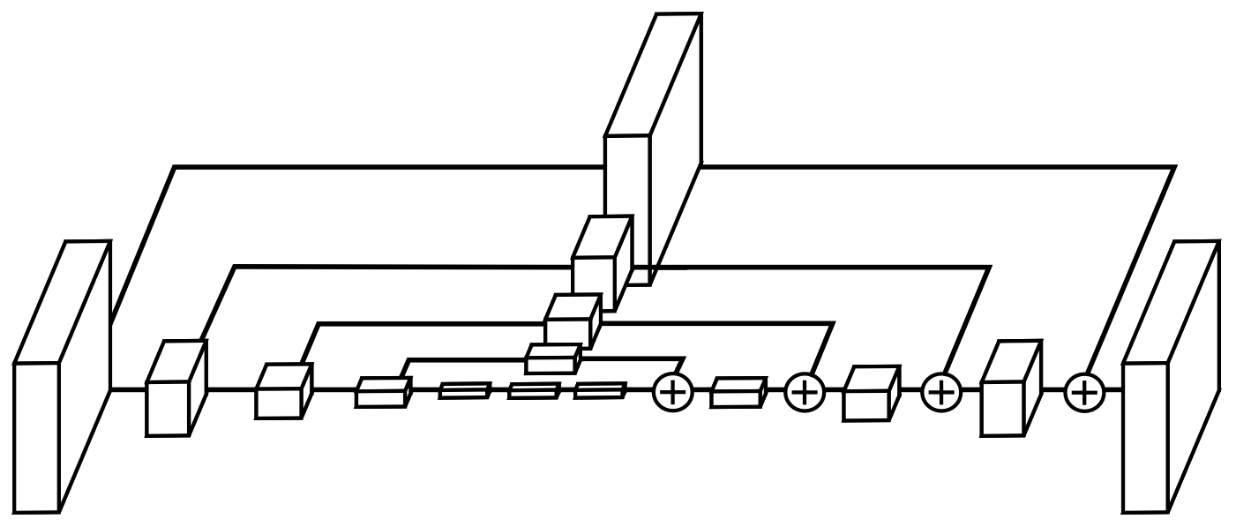
\includegraphics[width=\textwidth]{figures/sh.png}
    \caption{Diagram of a single \emph{Hourglass Module}, the main building block of the \emph{Stacked Hourglass} architecture proposed by Newell \etal\cite{Newell2016-cy}.}
    \label{fig:sh}
\end{figure}

It is worth mentioning that simply stacking \emph{Hourglass Modules} without intermediate supervision would never take the \gls{sh} model to its full potential. This intermediate supervision process is achieved by optimizing the \emph{Mean Squared Error} between the predicted heatmaps and their ground-truth after each module. As in \glspl{cpm}, the target heatmap is created by locating a bi-dimensional \emph{Gaussian} function on each joint location. During evaluation, input samples are cropped and then resized to 256x256 pixels.

\subsection{Chained Predictions}\label{subsec:cp}
The method proposed by Gkioxari \etal\cite{Gkioxari2016-ix} is based on \emph{sequence-to-sequence} models~\cite{sutskever2014sequence}, in which multiple output variables are predicted sequentially, \ie the prediction for a given output does not only depends on the input, but also on the previously predicted output variables. They propose an extension of this kind of models for more general structured outputs taking images as input and demonstrate its performance in human pose estimation, which is a clear example of structured prediction. In their model, the prediction for each body joint is dependent on all previously predicted joints, following a fixed ordering, which is determined according to detection rates yielded by an unchained \emph{feed-forward} net. In that way, the easier cases are processed first, while the harder ones take advantage of all the contextual information given by the previous detected joints. In Figure~\ref{subfig:cp_general}, a diagram showing the \glspl{cp} model can be found. Gkioxari \etal architecture is composed of two main blocks, an encoder that processes the input image with several convolutional operations (\gls{cnn}\textsubscript{x}), and a decoder composed of deconvolutional layers (\gls{cnn}\textsubscript{y}). The image encoded by the \gls{cnn}\textsubscript{x} is shared for every joint, while there is a single \gls{cnn}\textsubscript{y} block for each joint, which takes as input the encoded image and predictions from previous joints. The architecture of each of these blocks is presented in Figure~\ref{subfig:cp_particular}.

\begin{figure}[h]\centering
    \begin{subfigure}{0.41\textwidth}\centering
        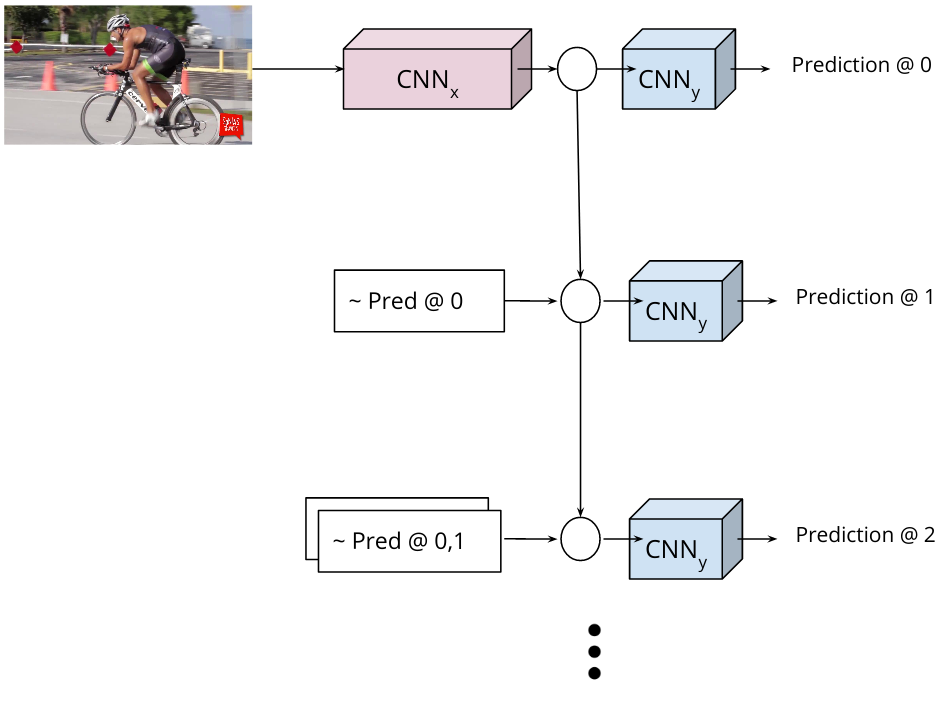
\includegraphics[height=5cm]{figures/cp_general.png} 
        \caption{CPs architecture.}
        \label{subfig:cp_general}
    \end{subfigure}
    \begin{subfigure}{0.58\textwidth}\centering
        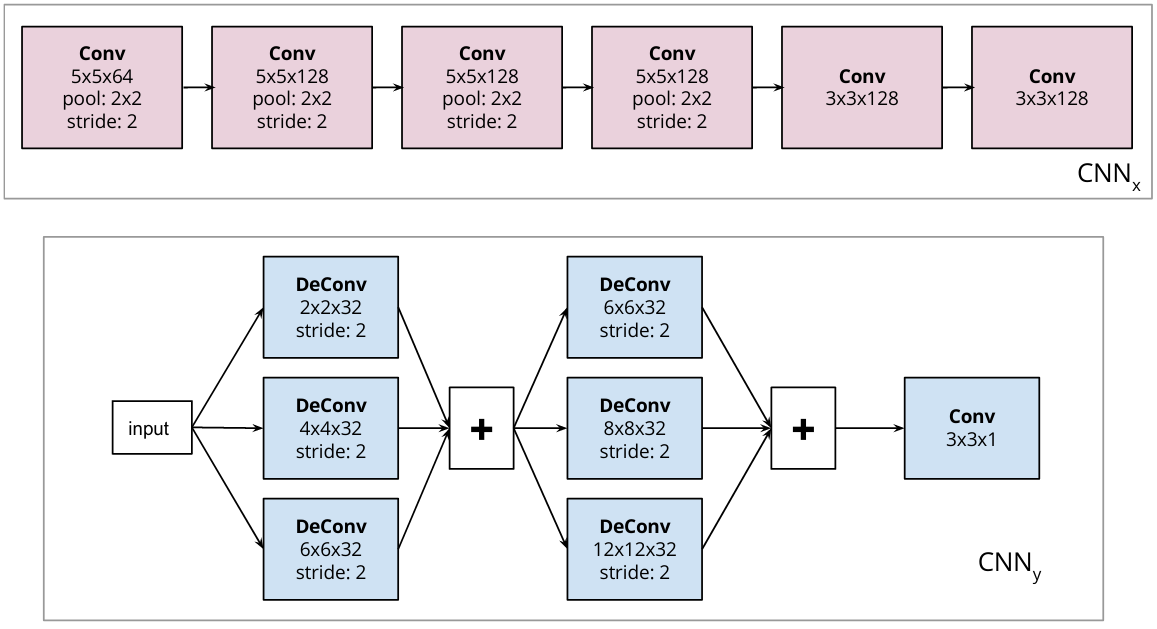
\includegraphics[height=5cm]{figures/cp_particular.png}
        \caption{Main CPs  model blocks.}
        \label{subfig:cp_particular}
    \end{subfigure}
    \caption{In (a), a complete diagram of the CPs architecture proposed by Gkioxari \etal\cite{Gkioxari2016-ix} is shown. The model proposed is composed of a single CNN\textsubscript{x} that encodes the input image, and several CNN\textsubscript{y} (decoders) which, taking as input the encoded image and the previous predictions, return a heatmap for each joint. Both blocks are shown in (b).}
    \label{fig:cp}
\end{figure}

During the first iterations of the training stage, the results from the previous joints predictions are replaced by their ground-truths, as these estimations can be really inaccurate and can jeopardize model convergence. Once the previous predictions start to get better, they are gradually introduced instead of their ground-truths. This training strategy is called \emph{scheduled sampling}, and was initially introduced by Bengio \etal\cite{bengio2015scheduled}. During evaluation, input samples are rescaled to 299x299 pixels.

\subsection{Conceptual comparison}\label{subsec:conceptual_comparison}
As it has been already mentioned, none of these methods are based on an explicit spatial model that takes into account the relation between each joint. Instead, these relations are implicitly learned  during training. In that way, the only model that makes an slight assumption regarding how each joint relates to each other is \glspl{cp}, which have a fixed order for its sequential prediction. However, even in that case, the order is previously decided by the accuracy obtained for each joint when estimating their locations using a \emph{feed-forward} net, so it is not imposed by any human decision.

Another shared key factor is that their training is performed \epmh{end-to-end}. The main difference then is how they manage to blend contextual information regarding other joints location and the input images. As stated in~\cite{Gkioxari2016-ix}, both \gls{sh} and \glspl{cpm} are based on an iterative process that gradually refines predictions, building up on very naive results in the first stages, while the \glspl{cp} model approach produces a single set of predictions, which are already quite accurate due to the imposed chained dependency.

The differences already mentioned set apart the \glspl{cp} model from the other methods described. Meanwhile, the key distinction between \gls{sh} and \glspl{cpm} can be found in the main building blocks of their architectures. While \gls{sh} is composed of multiple \emph{bottom-up} and \emph{top-down} subsequent stages, \glspl{cpm} further increase the receptive field of the model with each new stage. Besides that, \glspl{cpm} share weights across stages, while in~\cite{Newell2016-cy}, weights are not tied between each \emph{Hourglass Module} in any way.

\section{3D Estimation}\label{sec:3d_estimation}
Once 2D detection has been performed, the next step in our pipeline is the estimation of the 3D locations of the detected joints. For this task, we rely on image sequences captured with an RGBD sensor. We assume that color and depth images are registered, as most commercial sensors are coupled with \glspl{sdk} that provide their own calibration data and algorithms for that purpose. In this section, we present a detailed description of each step that composes our proposed method for 3D estimation. This method has been developed taking in mind the hard requirements imposed by robotics applications in terms of computational costs.

In Figure~\ref{fig:system_design}, an overview of the steps involved in the algorithm we propose for 3D estimation can be seen. Here is a brief overview of these sequential steps:
\begin{enumerate}
    \item Noise from depth image is reduced by filtering with a \emph{Gaussian} kernel.
    \item A minima filter centered at each 2D estimation over the depth image is used to ensure we are working with distances to the human subject in the foreground.
    \item Corrected 2D estimations and their corresponding depth are reprojected to get three-dimensional camera coordinates.
    \item Outliers in the resulting 3D keypoints are rejected.
    \item The final 3D estimation for each joint is given by a \emph{Kalman} filter that smooths the results leveraging temporal cues. It also provides estimations for the joints rejected in the previous step.
\end{enumerate}

\subsection{\emph{Gaussian} blur}\label{subsec:gaussian_filter}
\emph{Gaussian} blur is a basic tool widely used in computer vision for reducing noise in images, at the cost of losing high-frequency details. It is named after the mathematician Carl Friedrich Gauss. When working in the spatial domain, this filtering is equivalent to a convolution between the image and a two-dimensional \emph{Gaussian} function, defined as:

\begin{equation}
    G(x, y) = \frac{1}{2\pi\sigma^2}e^{-\frac{x^2 + y^2}{2\sigma^2}}
\end{equation}\label{eq:gaussian_blur}
where \(x\) and \(y\) represent the distance to the origin of the filter in each dimension and \(\sigma\) determine its standard deviation. 

Depth images are prone to contain a significant amount of noise, as they can be highly influenced by environmental factors. Such is the case of cameras that rely on projected light in the infrared domain, which can be influenced by sunlight, or even stereo cameras, which might fail to match pixels between images if the surface does not have enough salient points. Besides that, losing high-frequency details in the resulting depth estimations is not a major issue, as distance to camera is supposed to follow a smooth progression within the surface of the objects of interest in the scene. Applying a \textit{Gaussian} blur to the depth image alleviates the undesired effects mentioned above. 

In our case, we apply a kernel of size 5x5. The standard deviation is automatically computed from the given kernel size by \emph{OpenCV}~\cite{opencv_library}. In Figure~\ref{fig:gaussian_blur}, an example of a filtered depth map can be seen. It is important to note that the size of the kernel used for filtering is highly dependent on the image resolution and the size of the objects in the scene, so it might need some tuning depending on the particular application.

\begin{figure}[h]
    \centering
    \includesvg[width=\textwidth]{figures/gaussian_blur.svg}
    \caption{Naive example of a \emph{Gaussian} blur applied to a depth map.}
    \label{fig:gaussian_blur}
\end{figure}

\subsection{Minima filter}\label{subsec:minima_filter}
Besides the inherent noise in depth images, the 2D estimations provided by the methods described in Section~\ref{sec:2d_estimation} can be slightly displaced from the real joint location. Our next strategy for filtering out outliers in the depth estimation is a minima filter around the 2D detected region in the depth image. We choose a minima filter because we are retrieving spatial information from subjects who are consistently closer to the camera than the rest of the objects in the scene. Our minima filter is also useful if the pixel in the depth image for the detected 2D keypoint contains a null value, which is quite frequent in RGBD sensors. An example of how this technique can help filtering out noisy depth estimations is shown in Figure~\ref{fig:minima_filter}.

\begin{figure}[h]
    \centering
    \includesvg[width=\textwidth]{figures/minima_filter.svg}
    \caption{Minima filter over the detected 2D joint region can help filtering out noisy depth measurements.}
    \label{fig:minima_filter}
\end{figure}

We fix the initial kernel size for this minima filter to 11x11 pixels around each joint. Once again, this kernel size might depend on the image resolution and the size of the objects in the scene. Let \(D\) be our depth image and \(W_{x_j, y_j}\) a window of the depth image \(D\) with size 11x11 centered around the estimated 2D coordinates \(x_j, y_j\) for the $j$-th joint, we estimate its distance to the camera as
\begin{equation}
    z_j = min(W_{x_jy_j})
\end{equation}\label{eq:minima_filter}
Exceptionally, if no valid pixel is found in \(W_{x_j, y_j}\) due to corrupt data in \(D\), we increase the size of the filter until at least one valid pixel is found.

\subsection{Reprojection}\label{subsec:reprojection}
For reprojecting the estimated 2D coordinates into a three-dimensional space, we will use a pinhole camera model, which simplifies how a real camera works by assuming an infinitely small aperture and no lens. In our case, this is a reasonable assumption as most \glspl{sdk} provided by depth sensors manufacturers allow the user to correct the geometric distortions that the camera lens might have introduced in the image.

The image formation process for pinhole cameras can be described by its intrinsic and extrinsic matrices. The former describes the parameters of the system that are inherent to the camera itself, \ie its focal length in \(x\) and \(y\) dimensions (\(f_x, f_y\)) and the coordinates of its optical center (\(c_x, c_y\)). The latter includes a description of how the camera coordinates relate to the world coordinates, expressed as a three-dimensional rotation and translation matrix. In Figure~\ref{fig:projection}, we can see how all of these parameters are involved in the image formation process, from world coordinates to pixels in the final image.

\begin{figure}[h]
    \centering
    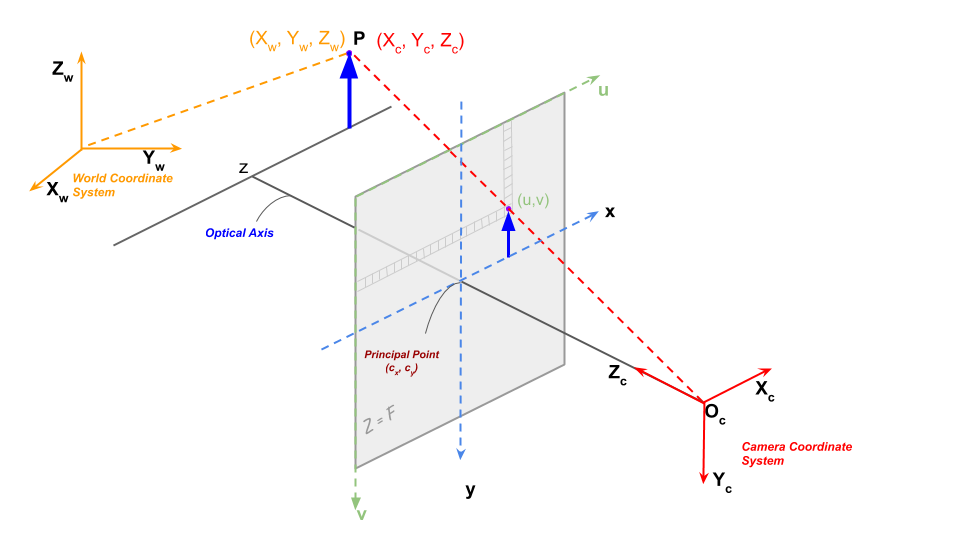
\includegraphics[width=\textwidth]{figures/projection.png}
    \caption{Projection of point \(P\) from world coordinates to camera, image and pixel coordinates, as modeled by a pinhole camera (source \cite{mallick_2020}).}
    \label{fig:projection}
\end{figure}

In our case, given the estimated distance to camera \(z_j\), image coordinates \(x_j, y_j\), depth image \(D\) dimensions \((w, h)\) and camera intrinsic parameters \(f_x, f_y, c_x, c_y\), we get the 3D camera coordinates of each joint \(j\) as:
\begin{equation}
    X_{j, cam} = \frac{(w - x_j - c_x) * z_j}{f_x}
\end{equation}\label{eq:3d_coordinates_x}
\begin{equation}
    Y_{j, cam} = \frac{(h - y_j - c_y) * z_j}{f_y}
\end{equation}\label{eq:3d_coordinates_y}
\begin{equation}
    Z_{j, cam} = z_j
\end{equation}\label{eq:3d_coordinates_z}
If extrinsic camera parameters are also provided, these camera coordinates can be projected to real-world coordinates. However, camera coordinates are enough for the performance evaluations and demos presented in this work.

\subsection{Outlier rejection}\label{subsec:outlier_rejection}
As we already mentioned in Section~\ref{subsec:minima_filter}, we might find outliers in our predicted 3D coordinates due to inconsistencies in the depth maps and noisy 2D estimations. Some of these outliers are so clear that they can be rejected with very intuitive sanity checks. It is important to note that simply rejecting these outliers would be unacceptable if no further processing was performed on the estimations. However, thanks to the \emph{Kalman} filtering presented in next section, we can replace rejected estimations for a joint with predictions yielded by its \emph{Kalman} filter based on results from previous frames.

For our application, we will consider two criteria for identifying outliers: based on the distance of the joints to the body center and based on their motion speed between consecutive frames.

\subsubsection{Based on distance to body center}
Taking as body center the estimated 3D coordinates for the pelvis center, we reject any joint with an estimated distance to that particular point higher than 150cm. This threshold has been imposed taking into account the common range of heights in adult humans (around 95\% of population height lies between 150 and 190cm~\cite{roser2013human}). We choose as reference the pelvis estimation as it is rarely occluded and, even if the estimation is a bit off, is very unusual to have strong deviations from its true location. In that way, we try to ensure a more robust outlier rejection.

\subsubsection{Based on per-joint velocity}
Another easy way to check whether a joint has been erroneously estimated or not is validating the amount of displacement between frames. We reject any joint with a displacement between frames higher than 50cm, \eg if we assume a frame rate of 20 \gls{fps}, that would be a velocity higher than 10m/s.

\subsection{\emph{Kalman} Filtering}\label{subsec:kalman_filtering}
Until this point of the process, human joints locations are estimated in a \emph{frame-by-frame} manner, without imposing any temporal dependency. In order to reduce noise and uncertainty in the 3D coordinates estimated by our method when applied to RGBD video sequences, we use an independent \emph{Kalman} filter~\cite{kalman1960new} for each joint in the skeleton.

\emph{Kalman} filters are a very powerful tool for filtering linear continuous data at a very low computational cost, both in terms of memory and time, which makes them suitable for embedded applications that must work in real-time. In a nutshell, they provide estimates of unknown or hidden variables given their uncertain measurements observed along time. Besides their lightweight implementation, another key advantage of \textit{Kalman} filters is that they do not need labeled training data of any kind to make their estimates. A great limitation of this algorithm is that for obtaining an optimal result, \textit{Gaussian} noise is assumed.

As it is shown in Figure~\ref{fig:kalman}, at each time step the algorithm performs two stages: prediction and update. During prediction, an estimate of the state of the variables defined is given depending on the physical model imposed by means of a transition matrix, the previous measurement and predictions and its uncertainty matrix. With each new measurement, both the state of the system and its uncertainty are updated and a new prediction is yielded. In our case, the state vector is formed by the three-dimensional location of each human joint estimated.

\begin{figure}[h]
    \centering
    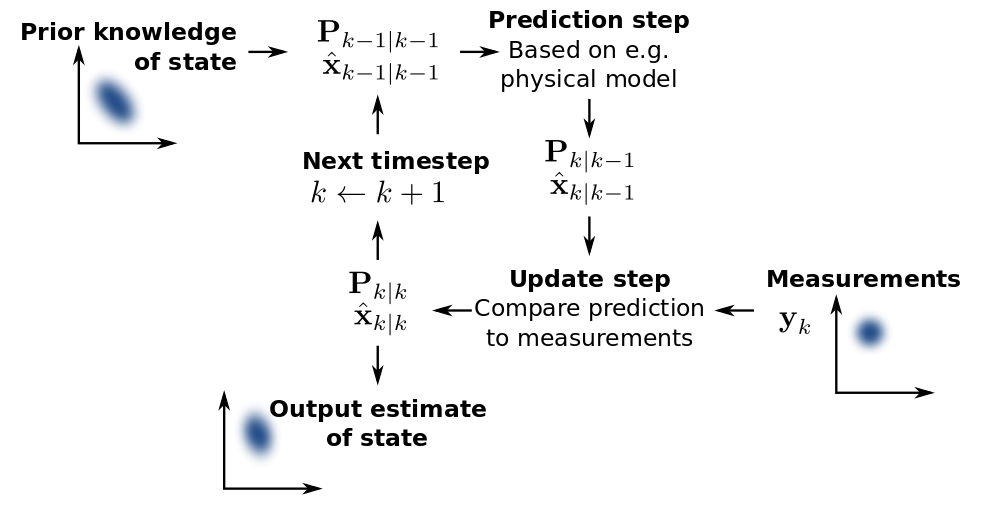
\includegraphics[width=\textwidth]{figures/kalman.png}
    \caption{Definition of the \emph{Kalman} filter algorithm in terms of its prediction and update stages~\cite{petteri_2011}.}
    \label{fig:kalman}
\end{figure}

In this work, we have used the \emph{pykalman} library for \emph{Python} for implementing \emph{Kalman} filters~\cite{pykalman}. It provides a very intuitive interface and allows returning predictions even if no new measurement is provided. We leverage this property for yielding new estimations for joints that have been marked as missing by our outlier rejection mechanisms. In order to avoid too much spatial drifting caused by these missing estimations, if no measurement is provided during \(n\) consecutive frames for a given joint, its \emph{Kalman} filter is reinitialized as soon as a new estimation is available. In our tests, we have set \(n\) to 4 frames.